\chapter{灵长类动物前额叶皮层的进化}

\section{概述}
前额皮层的进化经历了不同的阶段。早期哺乳动物经历了一次进化,产生了所有哺乳动物共有的颗粒状前额(后文简称PF)区域。这些区域的产生能根据预测结果改善行动(第3章)和对象(第4章)之间的觅食选择。
早期灵长类动物经历了另一个进化,形成了第一个颗粒状的PF区域。
原本这些动物的仅在夜间生活于细小的树枝上,它们在那里寻找、选择和获取食物,用一种需要头部和一只手协调运作的方法进食。
他们进化后的PF区域有助于根据当前的生物需求和特定的习惯(第4章)来选择食物,以及在杂乱的环境中保持对食物的注意力(第5章)。
后来,在类人猿灵长类动物的进化过程中,随着这些物种及其大脑体积的增加,出现了额外的颗粒状 PF 区域。
它们依靠最新进化的灵长类中央凹和改进的色觉在白天觅食。 因此,可以比它们的祖先更好地处理时空事件的顺序(第6章)并对资源的迹象进行检测(第7章)。
因为丰富的资源分散在类人猿的园区范围内,它们面临着严峻的资源波动、捕食和竞争问题。
他们的新 PF 区域使他们能够通过使用单一事件来选择觅食目标(第8章)来减少风险和非生产性觅食选择的数量。

\section{介绍}
本章探讨了颗粒状前额皮层在早期灵长类动物中首次出现的结果,以及仅灵长类动物拥有这种皮层的事实(Preuss 2007a)。

由于其名称,一些神经科学家认为关于颗粒状前额皮层的进化历史仅取决于生物的细胞结构。考虑到这一主张的重要性,有人可能会争辩说这是一个薄弱的支撑。幸运的是,许多其他特征支持了“颗粒状前额皮层在灵长类动物中的进化”这一观点。接下来,我们将列出其中的四个特征:皮层区域之间的空间布局、颗粒状前额皮层向纹状体的投射模式、感觉输入的分布、以及通过电刺激皮层引起的自主神经反应。

图2.1展示了我们对人类、猕猴和小白鼠这三个物种颗粒状前额皮层的同源性的看法,这主要归功于Preuss和Goldman-Rakic(1991a)的开创性工作。同源性指的是由于共同祖先的遗传而在相关物种中出现的类似区域。该图以浅灰色显示了仅在灵长类动物中进化出来的颗粒状前额皮层。这些颗粒状区域同样出现在人类和猕猴的大脑中,但不出现在老鼠的大脑中。老鼠只有无颗粒状前额皮层区域,该图为三个物种均以深灰色表示。我们选择这三个物种,是因为我们对前额皮层的大部分知识都基于对它们的大脑的研究。

\begin{figure}
	\centering
	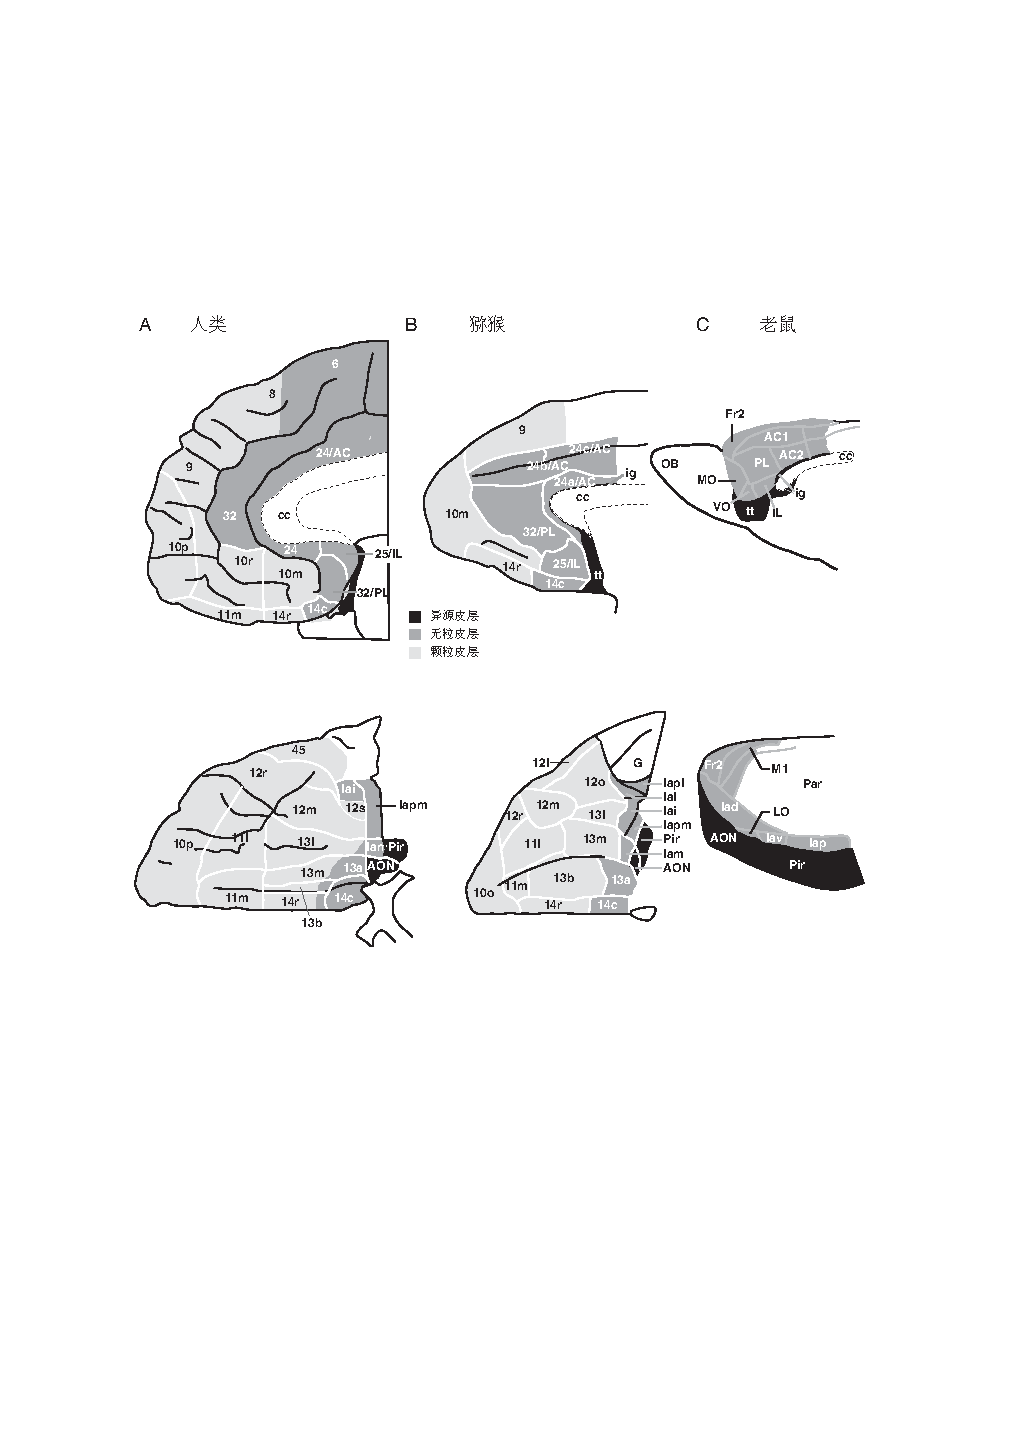
\includegraphics[width=0.7\linewidth]{image_pfc/Fig_2_1}
\end{figure}

图2.1(A)人类前额皮层的内侧(上)和眶上区(下)(Ongur等人,2003)。 (B)猕猴前额皮层的内侧(上)和眶上区(下)(Carmichael&Price,1994)。 (C)老鼠前额皮层的内侧(上)和侧面(下)(Palomero-Gallagher&Zilles,2004)。在所有图中,向左为前端。上行:所有图中背面向上。下行:(A)和(B)中,侧面向上;在(C)中,背面向上。不按比例。缩写:AC,前扣带皮层;AON,前嗅“核”;cc,胼胝体;Fr2,第二额区;la,不含颗粒的岛叶皮层;ig,灰脑层;IL,下极叶皮层;LO,外侧眶上皮层;MO,内侧眶上皮层;OB,嗅球;Pir,锥体(嗅觉)皮层;PL,前扣带区;tt,盖带;VO,腹侧眶上皮层。区域细分标记为尾部(c);下(i);侧面(l),内侧(m);眶上(o),后部或极端(p),前端(r),或按任意标记(a,b)。 (A)改编自Ongur D. Ferry AT,Price JL。《人类眶上和内侧前额皮层的建筑分区》,《比较神经解剖学杂志》460:425-49,©2003,经John Wiley和Sons许可使用。 (B)改编自Carmichael ST,Price JL.《猕猴颅内和眶上前额皮层的建筑分区》,《比较神经解剖学杂志》346:366-402,©1994,经John Wiley和Sons许可使用。 (C)改编自Palomero-Gallagher N,Zilles K.《大鼠神经系统》中的异皮层.ed.G Paxinos,pp.729-57.圣迭戈,加利福尼亚州:爱尔斯维尔学术出版社。

非颗粒性前额叶皮层区域包括下肢内侧皮层、前扣带皮层、无颗粒的岛叶皮层、无颗粒的眶上皮层和前扣带回。在不同物种中,这些区域往往有不同的名称。例如,啮齿动物的下肢内侧皮层与灵长类动物的25区大致相对应,von Bonin和Bailey将其称为FL区(图1.1)。

众所周知,许多神经科学家认为老鼠拥有与灵长类动物相同的前额叶皮层。并且他们坚持认为,老鼠具有模拟灵长类动物前额叶皮层的微型复制品,或者可以将其所有属性混合在他们的小型无颗粒区域中(Kolb 2007;Seamans等人2008;Schoenbaum等人2009)。虽然我们对此持有不同的观点,但有一个命题应该得到普遍接受:在进化历史的某个时刻,我们的某些祖先缺乏颗粒性前额叶皮层。然而,现在我们不再缺失它。鉴于这个历史事实,询问颗粒性前额叶皮层带来了什么优势似乎是合理的。

尽管不是每个人都同意图2.1所描绘的同源性,但没有人严肃地质疑现代啮齿动物的大脑缺乏颗粒状前额叶皮层这一事实。对于其他哺乳动物,有一点存在争议:有人认为狗(Rajkowska&Kosmal 1988)和猫(Rose&Woolsey 1948)具有颗粒状前额叶皮层区域。但当我们亲自检查组织学材料中,狗和猫所谓的颗粒状区域时,它们看起来很像猴子和啮齿动物的无颗粒区域。

正如第1章所述,这种争议可能是由于观察者缺乏成体系的知识方法所致。当Mackey和Petrides(2010年)在猕猴和人脑中观察到这个问题时,他们发现一些传统上被归类为无颗粒额叶区域的区域实际上在第4层细胞体密度上,与最尾端的区域相比有略微的增加。也就是说,这些区域具有较弱的非颗粒质细胞结构,而不是完全的无颗粒结构。在食肉动物和其他非灵长类哺乳动物中发现颗粒状PF皮层的报告,反映了这种属性。神经解剖学家们都认为,细胞从额叶轨道和内侧表面向头部移动时,第4层的厚度会持续增加。因此,无颗粒皮质是否在第4层完全消失并不重要。我们可以将第4层密度低于给定阈值的区域视为足够无颗粒这一标准,用于我们之后的研究中(如图2.2所示)。

尽管大鼠缺乏细颗粒前额皮层,但一些神经科学家仍认为,大鼠前额皮质的中部与灵长类动物的中侧颗粒前额皮层(区域46)同源(Kolb 2007; Seamans等,2008),尽管后者的是一个颗粒区域(也称为背外侧或周主前额皮层)。同样,还有一些人认为,大鼠前额皮质的侧部与灵长类动物的整个眶前颞皮质同源,包括其颗粒部分(Kolb 2007; Schoenbaum等,2009)。该论点基于解剖学、生理学和神经化学的相似性以及基于声称在老鼠和猕猴中的损伤效应的相似性。

\begin{figure}
	\centering
	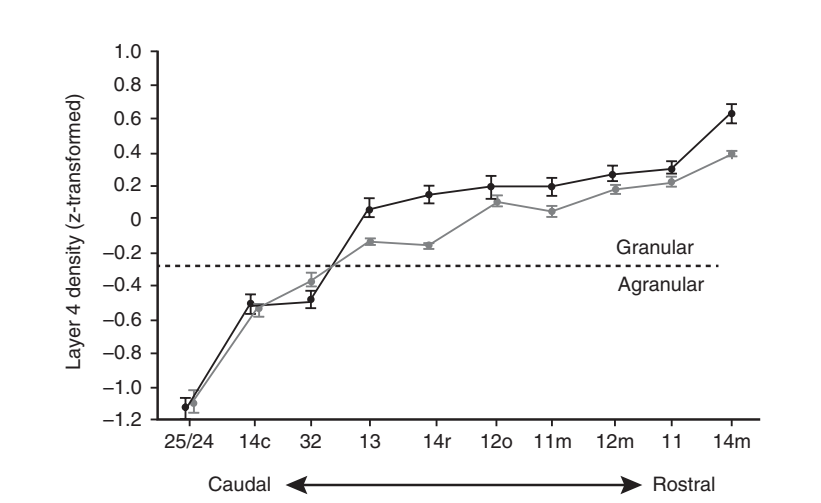
\includegraphics[width=0.7\linewidth]{image_pfc/Fig_2_2}
\end{figure}

图2.2 显示了大脑额叶区域从尾向头发展的过程中,第4细胞层的归一化密度在猕猴(黑线)和人类(灰线)中的变化。误差条:SEM。该图由 Mackey S、Petrides M. 在《欧洲神经科学杂志》2010年32期(1940-1950页)中发表,经John Wiley and Sons出版社许可后再版。该图表明人类和猕猴大脑的腹内侧和侧壁眶前额皮质中具有可比较的成系统的区域。

然而,人们不能仅仅依据常被引用的相似性就推断其同源性。正如 Preuss(1995)所解释的那样,人们需要对特征进行诊断,即区分一组皮层区域和其他区域的特征区别。例如,老鼠的非颗粒状前额皮质与猕猴的颗粒状前额皮质区域具有许多相似之处,例如编码估值的细胞。但是,这三个区域——老鼠的非颗粒状前额皮质以及猕猴的非颗粒状和颗粒状前额皮质——都具有上述同样的特性,其他皮层区域也是如此。因此,它们无法帮助我们理解前额皮层皮质的进化或建立其区域之间的同源性。例如,老鼠的非颗粒状区域的特性与灵长类动物的颗粒状前额皮质相似,但它们也与灵长类动物的非颗粒状前额皮质相似,那么这些特性就与动物的同源性无关。

一些人声称与丘脑中背内侧核(MD)的连接是颗粒状前额皮质的诊断特征(Rose&Woolsey 1948;Akert 1964;Uylings等,2003)。但是,MD核向几乎所有的额叶投射,包括颗粒状和非颗粒状区域。因此,是否与MD核的连接不能作为诊断特征,故对同源性问题几乎没有影响。

曾经有一段时间,人们认为多巴胺能输入是颗粒状前额皮质的特征(Divac等,1978;Porrino&Goldman-Rakic,1982)。但是这些输入也终止于PF皮质的非颗粒状部分和运动前区,以及额叶以外大部分皮质。事实上,在灵长类动物中,多巴胺输入到运动前皮质和后枕叶皮质的强度比大多数颗粒状前额皮质都要强(Gaspar等,1992;Williams&Goldman-Rakic,1998)。因此,多巴胺输入不能帮助我们跨物种识别PF皮质。

